\documentclass[11pt,a4paper]{article}

\usepackage[T1]{fontenc}
\usepackage[utf8]{inputenc}
\usepackage[english]{babel}
\usepackage[a4paper,margin=2.0cm]{geometry}
\usepackage{amsmath,amssymb,amsfonts}
\usepackage{graphicx}
\usepackage{booktabs}
\usepackage{float}
\usepackage{hyperref}
\usepackage{enumitem}

\graphicspath{{../figures/}}
\setlength{\parindent}{0pt}
\setlength{\parskip}{3pt}
\setlength{\emergencystretch}{2em}
\setlist[itemize]{noitemsep, topsep=2pt, leftmargin=*}

\hypersetup{
    colorlinks=true,
    linkcolor=blue,
    urlcolor=blue,
    citecolor=blue
}

\newcommand{\R}{\mathbb{R}}
\newcommand{\norm}[1]{\left\lVert #1 \right\rVert}

\title{Cooperative Kernel Regression\\
\large Distributed Optimization, Federated Learning, and Differential Privacy}
\author{Agathe PASCAL & Nastassia BONETTI}
\date{\today}

\begin{document}

\maketitle

\begin{abstract}
This report presents a course-consistent implementation of Gaussian-kernel ridge regression with a Nyström approximation.
The experiments cover distributed optimization over a communication graph, federated learning, and a differentially private distributed variant.
The focus is on the mathematical formulation, stable parameter choices, convergence plots, and a concise interpretation of the observed behavior of each method.
\end{abstract}

\section{Common formulation}

The kernel is
\[
k(x,\xi)=\exp\left(-(x-\xi)^2\right).
\]
Given $n$ samples $(x_i,y_i)$ and $m$ Nyström landmarks $\tilde x_1,\dots,\tilde x_m$, define
\[
(K_{mm})_{pq}=k(\tilde x_p,\tilde x_q),
\qquad
(K_{nm})_{ip}=k(x_i,\tilde x_p).
\]

The centralized problem is
\[
\alpha^\star \in \arg\min_{\alpha\in\R^m}
\frac{\sigma^2}{2}\alpha^\top K_{mm}\alpha
\;+\;
\frac12\norm{y-K_{nm}\alpha}^2
\;+\;
\frac{\nu}{2}\norm{\alpha}^2,
\]
with $\sigma=0.5$ and $\nu=1$. Since the objective is quadratic and strongly convex,
\[
\alpha^\star=
\left(K_{nm}^\top K_{nm}+\sigma^2K_{mm}+\nu I_m\right)^{-1}K_{nm}^\top y.
\]
This solution is used as the reference point throughout the experiments.

\begin{figure}[H]
\centering
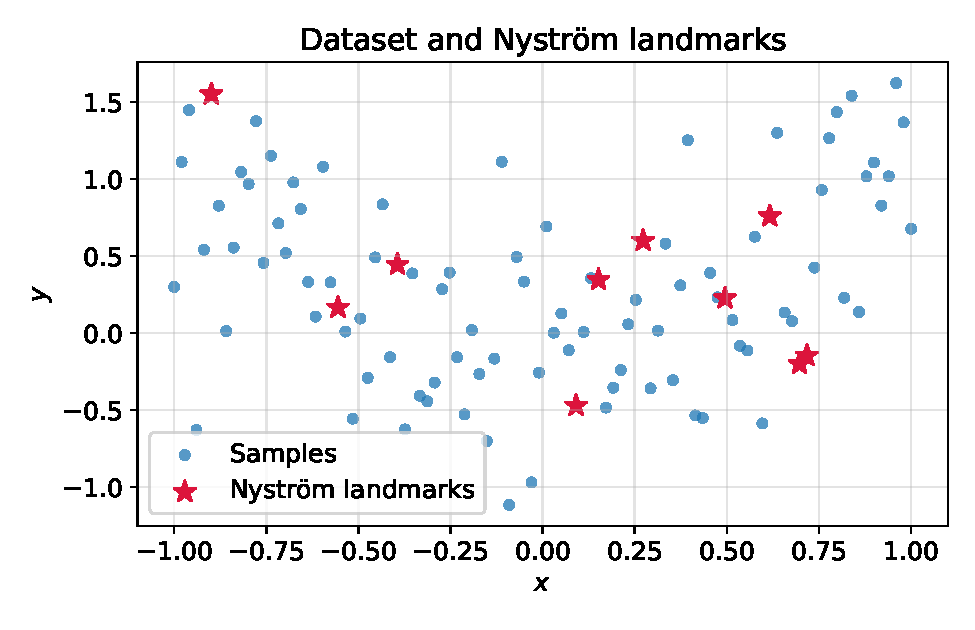
\includegraphics[width=.72\linewidth]{part1_dataset.pdf}
\caption{Samples used in Parts I and III, together with the selected $m=10$ Nyström landmarks.}
\label{fig:data}
\end{figure}

For the distributed setting, the first $n=100$ points are split over $a=5$ agents, hence 20 points per agent. With local data $(K_i,y_i)$ at agent $i$,
\[
f_i(\alpha)=
\frac{\sigma^2}{2a}\alpha^\top K_{mm}\alpha
\;+\;
\frac12\norm{y_i-K_i\alpha}^2
\;+\;
\frac{\nu}{2a}\norm{\alpha}^2,
\qquad
\sum_{i=1}^a f_i(\alpha)=F(\alpha).
\]
We monitor
\[
g_i^t=\norm{\alpha_i^t-\alpha^\star},
\qquad
\bar g^t=\norm{\bar\alpha^t-\alpha^\star},
\qquad
\bar\alpha^t=\frac1a\sum_{i=1}^a \alpha_i^t.
\]

\section{Distributed optimization}

Four graphs are tested: cycle, line, small-world, and complete. The undirected mixing matrices are built with Metropolis weights, so the standard course assumptions hold: symmetry, stochasticity, and connectivity.

The methods are DGD, Gradient Tracking (GT), dual decomposition, and ADMM. Their parameters are chosen from the local objective constants
\[
L_{\max}=\max_i \lambda_{\max}(H_i),
\qquad
\mu_{\min}=\min_i \lambda_{\min}(H_i),
\]
the graph mixing factor $\beta=\norm{W-J}_2$, and for the dual method
\[
L_d=\norm{B^\top H^{-1}B}_2.
\]

\begin{itemize}
\item \textbf{DGD:} \(\eta_{\mathrm{DGD}}=\min\!\left(0.9\frac{1-\beta}{L_{\max}},\,0.9\frac{1}{L_{\max}}\right)\). This keeps the method in the stable \(O((1-\beta)/L)\) regime. With a constant step size, DGD converges linearly to a neighborhood of \(\alpha^\star\) because the consensus error does not vanish exactly.
\item \textbf{Gradient Tracking:} \(\eta_{\mathrm{GT}}=0.2/L_{\max}\). The tracking variable reconstructs the global average gradient; under smoothness and strong convexity, a small enough \(O(1/L)\) step yields exact linear convergence.
\item \textbf{Dual decomposition:} \(\tau_{\mathrm{dual}}=1/(2L_d)\). The dual objective is smooth and concave, so this is a conservative stable ascent step that leads here to the exact solution.
\item \textbf{ADMM:} \(\rho_{\mathrm{ADMM}}=\sqrt{\mu_{\min}L_{\max}}\). In quadratic consensus problems, any \(\rho>0\) gives the exact solution; this choice balances the primal and dual scales.
\end{itemize}

\begin{figure}[H]
\centering
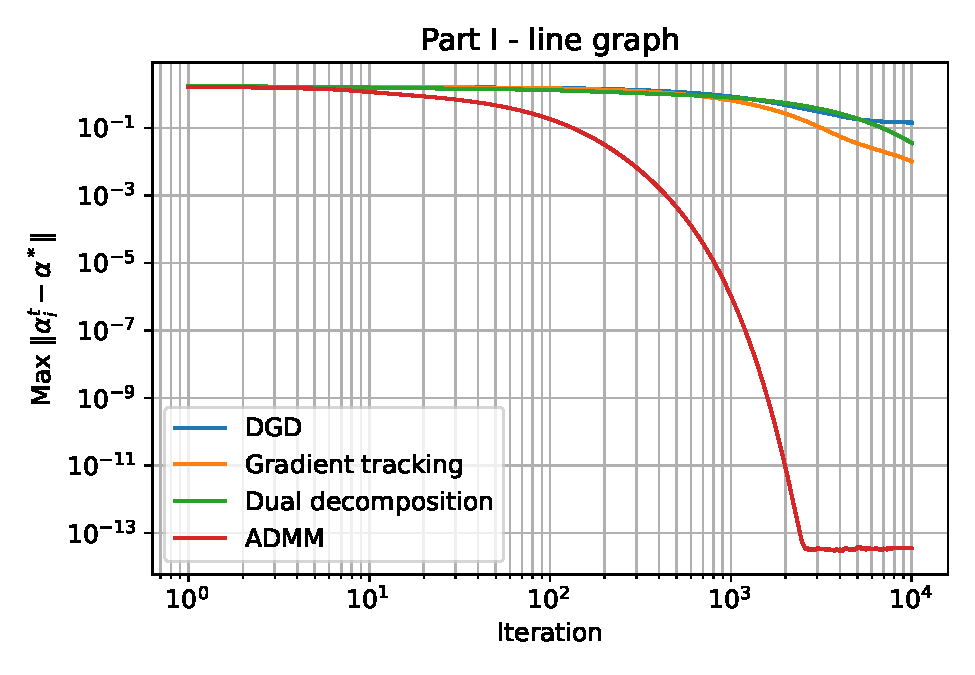
\includegraphics[width=.92\linewidth]{part1_gap_line.pdf}
\caption{On the line graph, DGD converges to a neighborhood of the solution, whereas GT, dual decomposition, and ADMM reach numerical precision.}
\label{fig:line}
\end{figure}

The line graph is representative: the worst final DGD gap is \(7.93\times 10^{-2}\), while the three other methods end below \(4\times 10^{-13}\). This matches the theory exactly: DGD with a constant step retains a consensus bias, whereas GT, the dual method, and ADMM are exact methods in this quadratic setting.

\begin{figure}[H]
\centering
\begin{minipage}[t]{0.48\linewidth}
\centering
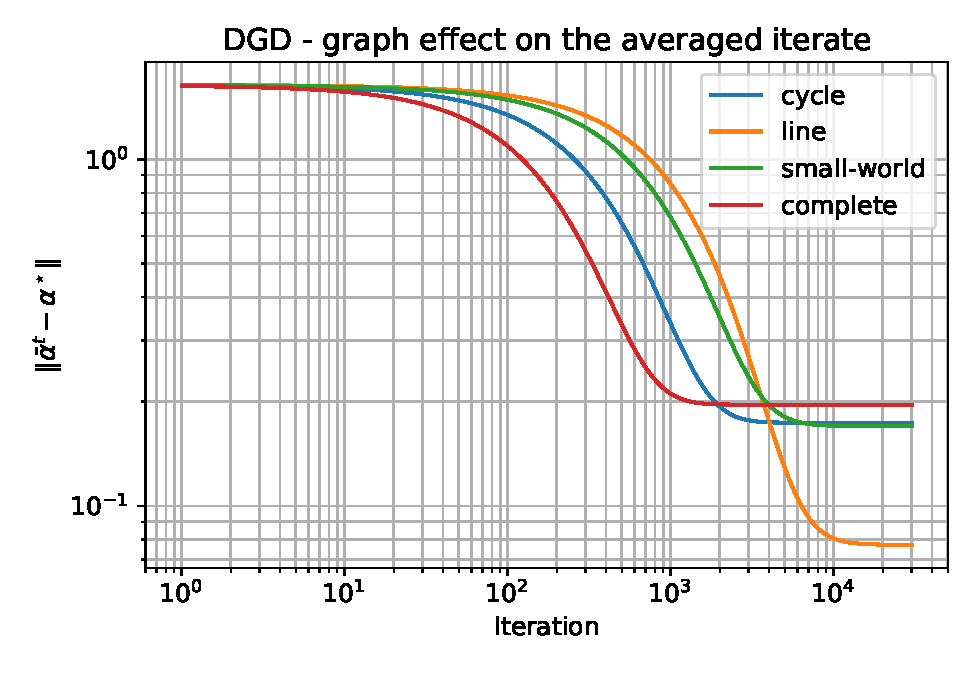
\includegraphics[width=\linewidth]{part1_dgd_graph_compare.pdf}
\end{minipage}
\hfill
\begin{minipage}[t]{0.48\linewidth}
\centering
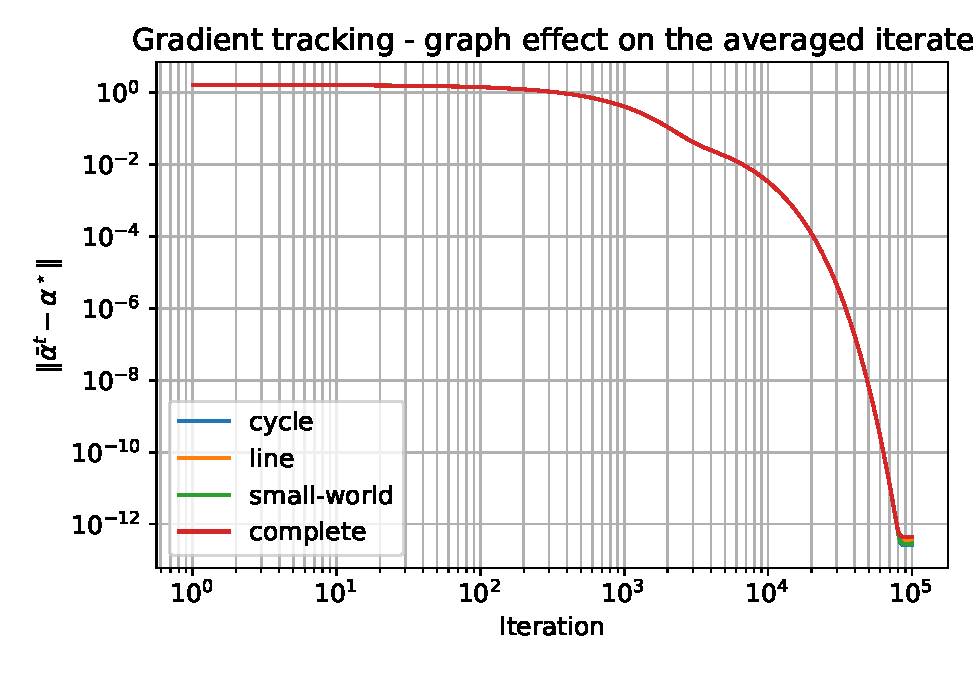
\includegraphics[width=\linewidth]{part1_gt_graph_compare.pdf}
\end{minipage}
\caption{Influence of the graph topology on the averaged iterate for DGD (left) and GT (right).}
\label{fig:graph_compare}
\end{figure}

Topology affects the methods differently. For DGD, better mixing mostly improves the transient phase and allows a larger admissible step; because \(\eta_{\mathrm{DGD}}\propto (1-\beta)/L_{\max}\), the final bias is therefore not strictly monotone in \(\beta\). For GT, the curves align much faster and all end at machine precision, confirming that the tracking term removes the steady-state bias observed in DGD. Dual decomposition and ADMM also reach the exact solution here because the consensus problem is quadratic, strongly convex, and solved through closed-form local updates.

\section{Federated learning}

The second dataset contains five clients with 20 points each. The global objective keeps the same Nyström structure:
\[
F(\alpha)=
\sum_{c=1}^5 \frac12\norm{y_c-K_c\alpha}^2
\;+\;
\frac{\sigma^2}{2}\alpha^\top K_{mm}\alpha
\;+\;
\frac{\nu}{2}\norm{\alpha}^2.
\]
The local mini-batch gradient used by FedAvg and SCAFFOLD is unbiased:
\[
g_{c,b}(\alpha)=
\frac{n_c}{|b|}K_{c,b}^\top(K_{c,b}\alpha-y_{c,b})
\;+\;
\frac{\sigma^2}{5}K_{mm}\alpha
\;+\;
\frac{\nu}{5}\alpha.
\]

The baseline local step size is
\[
\eta_{\mathrm{FedAvg}}=\frac{0.25}{L_{\max}^{\mathrm{loc}}}=3.136\times 10^{-3}.
\]
This keeps the local updates in a stable \(O(1/L)\) regime. When \(E=50\), the step is halved to limit client drift, which naturally grows with the number of local epochs between two aggregations.

\begin{figure}[H]
\centering
\begin{minipage}[t]{0.49\linewidth}
\centering
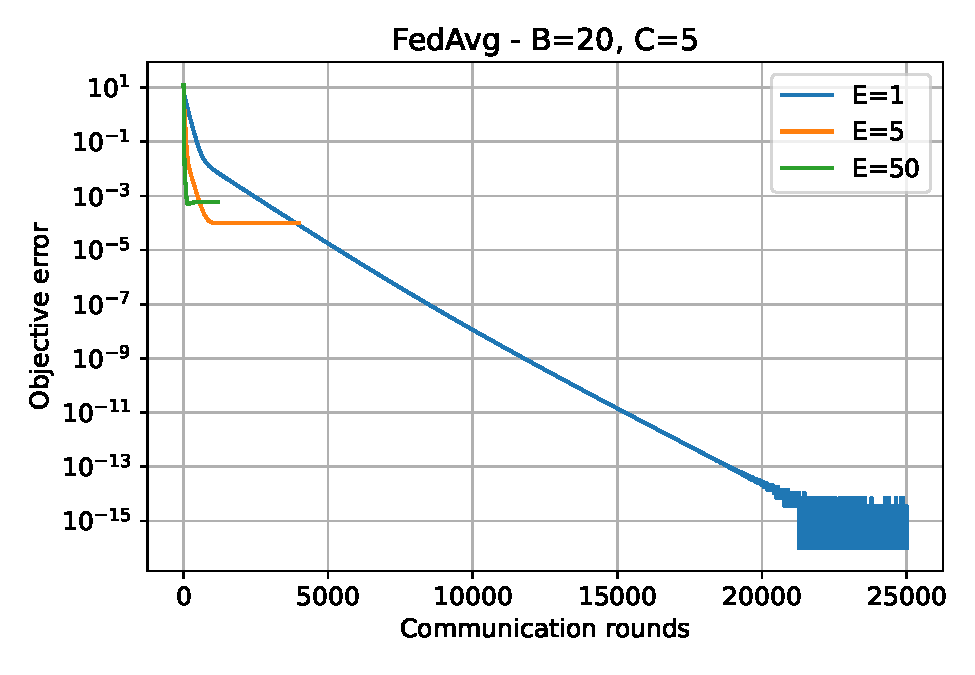
\includegraphics[width=\linewidth]{part2_fedavg_required_E.pdf}
\end{minipage}
\hfill
\begin{minipage}[t]{0.49\linewidth}
\centering
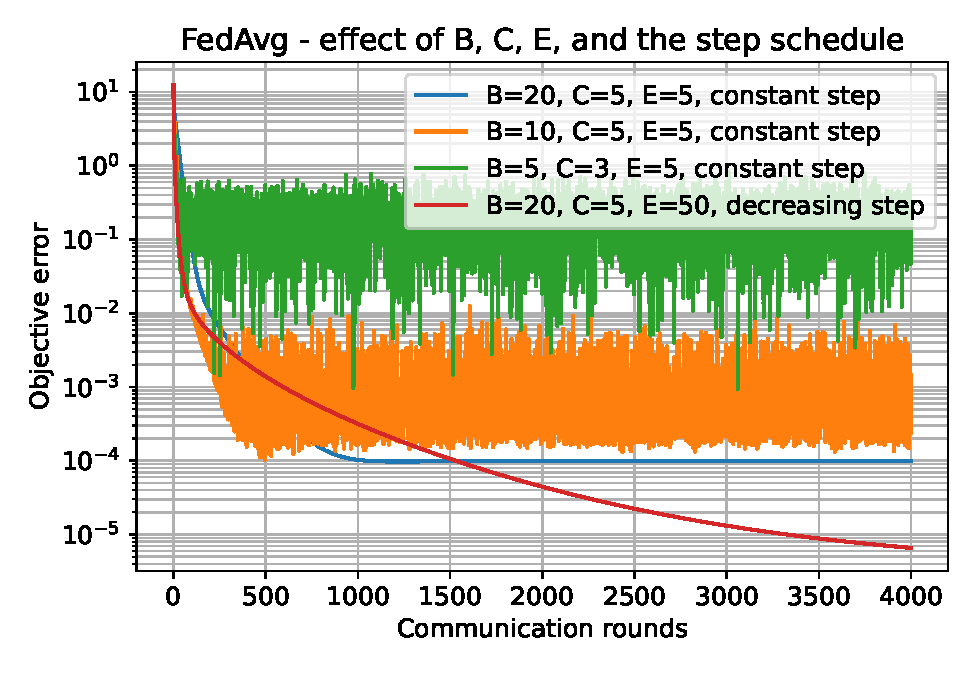
\includegraphics[width=\linewidth]{part2_fedavg_param_sweep.pdf}
\end{minipage}
\caption{FedAvg with \(B=20, C=5, E\in\{1,5,50\}\) (left), and the effect of \(B\), \(C\), \(E\), and the step schedule (right).}
\label{fig:fedavg}
\end{figure}

The results display the usual trade-off. For \(E=50\), descent per communication round is fast, but it requires a more cautious step size. For \(E=1\), the trajectory is much slower in communication rounds, yet it also reaches machine precision when the horizon is long enough. In the displayed runs, the final objective errors are \(<10^{-15}\) for \(E=1\), \(1.00\times 10^{-4}\) for \(E=5\), and \(5.81\times 10^{-4}\) for \(E=50\). The sensitivity plot confirms that decreasing \(B\) increases local variance, decreasing \(C\) slows down the global correction, and a decreasing step is mainly useful in the most aggressive settings.

The optional comparison with SCAFFOLD, run with \(C=3\) and \(E=5\), gives a final error \(2.03\times 10^{-2}\) for FedAvg versus \(2.13\times 10^{-14}\) for SCAFFOLD. This is consistent with the theory: the control variates compensate for client drift and become especially useful as soon as not all clients participate at every round.

\section{Differential privacy}

The private update reuses DGD on the line graph:
\[
\alpha^{t+1}=W\alpha^t-\eta\bigl(\tilde g^t+\xi^t\bigr),
\]
where \(\tilde g_i^t\) is the clipped local gradient and \(\xi_i^t\sim\mathcal N(0,\sigma_{\mathrm{DP}}^2I)\). Clipping is defined by
\[
\tilde g_i^t=g_i^t \min\!\left(1,\frac{c}{\norm{g_i^t}}\right),
\qquad c=5,
\]
which bounds sensitivity, and the Gaussian noise is calibrated as
\[
\sigma_{\mathrm{DP}}=\frac{2c\sqrt{2\log(1.25/\delta)}}{\epsilon\sqrt{T}},
\qquad
\delta=10^{-5}.
\]
The step size is kept equal to the deterministic DGD step on the line graph,
\[
\eta_{\mathrm{DP}}=8.693\times 10^{-4},
\]
so that different privacy levels are compared under the same stability condition. With a constant step and additive Gaussian noise, exact convergence is not expected; instead, the method should stabilize in a neighborhood whose size increases with \(\sigma_{\mathrm{DP}}\).

\begin{figure}[H]
\centering
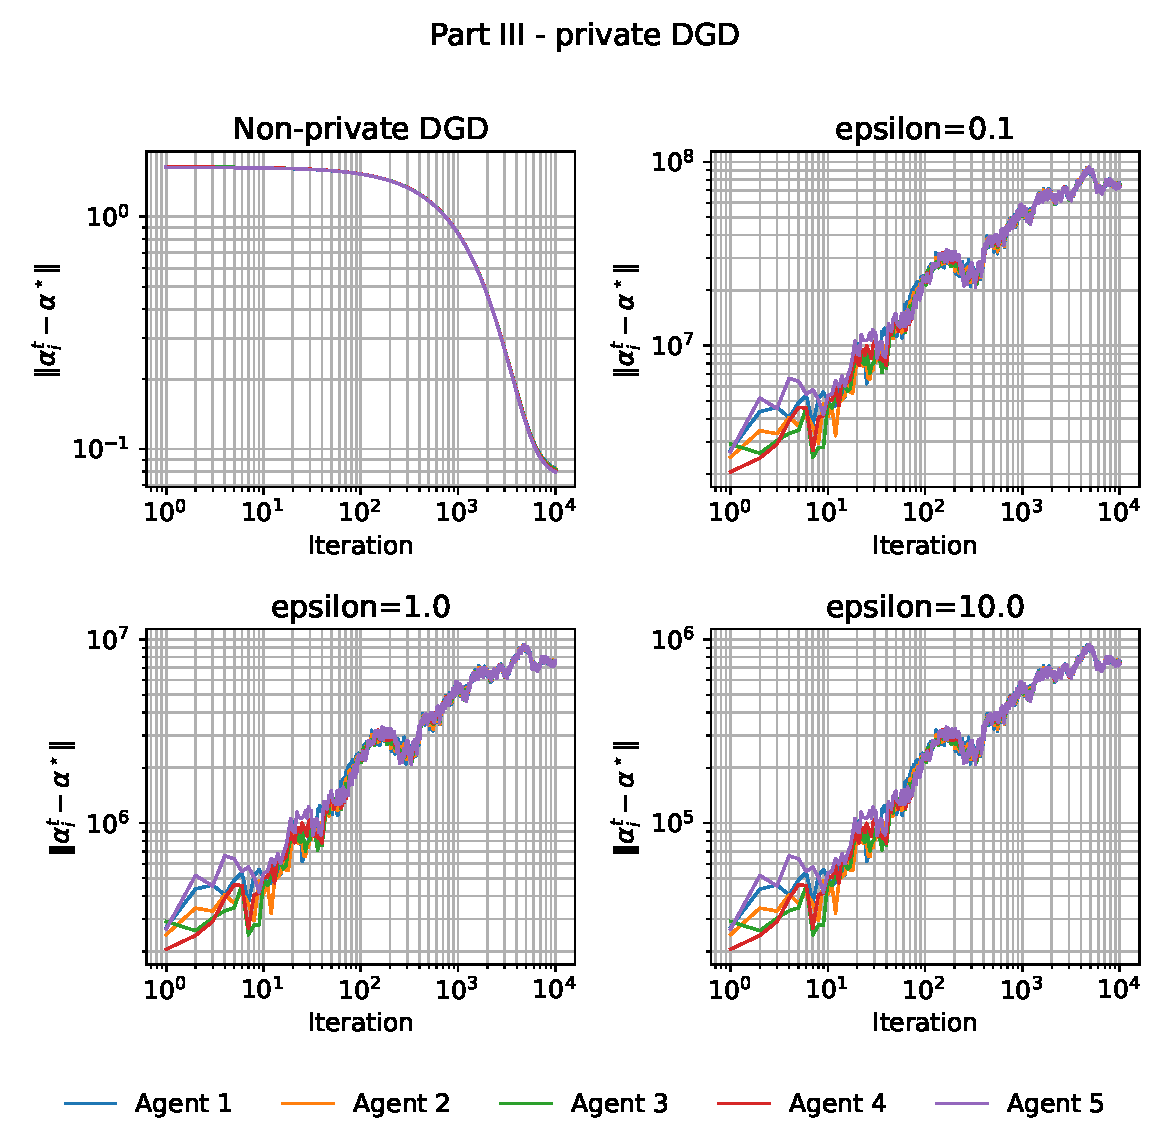
\includegraphics[width=.92\linewidth]{part3_dgd_dp_epsilons.pdf}
\caption{Agent-wise gaps for non-private DGD and private DGD with \(\epsilon\in\{0.1,1,10\}\).}
\label{fig:dp}
\end{figure}

The final gap of non-private DGD is \(8.05\times 10^{-2}\). The private variants stabilize around \(3.12\times 10^{-1}\), \(3.13\times 10^{-1}\), and \(3.20\times 10^{-1}\) for \(\epsilon=0.1,1,10\). The difference between the three privacy levels remains moderate in the displayed curves, not because privacy is free, but because the intrinsic DGD bias on the line graph is already a significant component of the total error. In other words, the observed plateau is dominated here by the combination \emph{consensus bias + privacy noise}.

\section{Conclusion}

The experiments support the following conclusions:
\begin{itemize}
\item the Nyström kernel-ridge formulation is used consistently across the three parts, with the centralized solution as the reference point;
\item in distributed optimization, DGD keeps a constant-step bias, whereas GT, dual decomposition, and ADMM converge exactly in this quadratic setting;
\item in federated learning, increasing the number of local epochs speeds up progress per round but also increases client drift, and SCAFFOLD corrects that drift effectively;
\item in differential privacy, DGD-DP remains stable but converges to a neighborhood, as expected with Gaussian noise and a constant step.
\end{itemize}

The numerical behavior is therefore coherent with the course notation and with the expected mechanisms of the different algorithms.

\end{document}
